% !TEX root = main.tex
% DIGT2107 — Iteration 2 document for OpenBid

\documentclass[11pt]{article}

% ---------- Basics (portable) ----------
\usepackage[margin=1in]{geometry}
\usepackage[T1]{fontenc}
\usepackage[utf8]{inputenc}
\usepackage{lmodern}
\usepackage{microtype}
\usepackage{xcolor}
\usepackage{hyperref}
\usepackage{enumitem}
\usepackage{booktabs}
\usepackage{longtable}
\usepackage{listings}
\usepackage{parskip}
\usepackage{graphicx}
\usepackage{float}
\usepackage{caption}

\hypersetup{
  colorlinks=true,
  linkcolor=black,
  urlcolor=blue!60!black,
  citecolor=black
}

% ---------- Listings ----------
\lstset{
  basicstyle=\ttfamily\small,
  columns=fullflexible,
  breaklines=true,
  frame=single,
  framerule=0.2pt,
  tabsize=2,
  showstringspaces=false
}

% Minimal JSON highlighting for listings
\lstdefinelanguage{json}{
  basicstyle=\ttfamily\small,
  numbers=left,
  numberstyle=\tiny,
  stepnumber=1,
  numbersep=8pt,
  showstringspaces=false,
  breaklines=true,
  frame=single,
  literate=
   *{0}{{0}}{1}{1}{{1}}{1}{2}{{2}}{1}{3}{{3}}{1}{4}{{4}}{1}
    {5}{{5}}{1}{6}{{6}}{1}{7}{{7}}{1}{8}{{8}}{1}{9}{{9}}{1}
    {:}{{:}}{1}{,}{{,}}{1}{\{}{{\{}}{1}{\}}{{\}}}{1}
    {[}{{[}}{1}{]}{{]}}{1}
}

% ---------- Title ----------
\newcommand{\course}{DIGT2107: Practice of Software Development}
\newcommand{\iteration}{Project Iteration 2: Detailed User Stories, Requirements, and Initial Prototype}
\newcommand{\project}{OpenBid}
\newcommand{\instructor}{Dr.\ May Haidar}
\newcommand{\duedate}{October 5, 2025}
\newcommand{\teamnum}{1}
\newcommand{\teammates}{Tyler, Mani, Yanness, Alaister}

\title{\course\\\large \iteration\\[6pt]\project}
\author{\teammates}
\date{\duedate}

\begin{document}
\maketitle

\begin{center}
\textbf{Course:} DIGT2107 -- Fall/Winter Term 2025-2026 \quad|\quad \textbf{Instructor:} \instructor \quad|\quad \textbf{Team:} \textbf{\#\teamnum}
\end{center}

\newpage

% ===================== 1. Introduction =====================
\section{Introduction}
\textbf{Project Name:} \project\\
\textbf{Team Number:} \textbf{\#\teamnum}\\
\textbf{Team Members:} \teammates

\paragraph{Document Overview}
This document outlines the deliverables for Iteration~2 of \project: detailed user stories, functional and non-functional requirements. The aim is to establish a solid foundation for subsequent iterations by clarifying what the system should do and validating the core experience with a working prototype.

% ===================== 2. Requirements =====================
\section{Functional and Non-Functional Requirements}

\subsection{Functional Requirements}
\begin{enumerate}[leftmargin=1.4em]
  \item \textbf{Account \& Identity:} Users shall be able to sign up and sign in via OAuth (Google/Apple) and email+password. Mandatory KYC must be completed before Contractors can publish profiles or Bidders can place offers.
  \item \textbf{Two-Factor Authentication (2FA):} Users shall confirm sign-in with Duo 2FA for sensitive actions (login, payouts).
  \item \textbf{Contractor Profiles:} Contractors shall create, update, and delete professional profiles with details including skills, description, photos, rate (fixed/hourly), availability, and location (map pin/address).
  \item \textbf{Discovery:} Bidders shall browse Contractors in list and map views, with filters by radius, category/skill, budget range, and availability date.
  \item \textbf{Bidding:} Job bidders shall place, edit, and withdraw bids (amount, note, ETA). Contractors shall accept a winning bid.
  \item \textbf{Payments (Escrow):}  When a Contractor accepts an offer, the Bidder shall fund an escrow hold. On job completion, funds shall be captured and paid out to the Contractor via Stripe Connect.
  \item \textbf{Messaging:} Contractors and Bidders shall exchange secure messages within the context of an offer, with support for attachments and report/block controls.
  \item \textbf{Reviews:} Both parties shall leave ratings and text reviews after completion.
  \item \textbf{Safety Score:} The system shall compute a location safety score (0--100) and apply graduated friction (tips, daylight default, verified-only, or manual review).
  \item \textbf{Admin:} Admins shall review reports, manage categories, and handle disputes via a basic dashboard.
\end{enumerate}

\subsection{Non-Functional Requirements}
\begin{itemize}[leftmargin=1.4em]
  \item \textbf{Performance:} Map/list browse and search shall return results in \(\leq 500\) ms p95 for target metro; prototype may use simplified filters.
  \item \textbf{Usability:} Mobile-first, accessible (WCAG 2.1 AA where practical); clear copy for KYC/2FA and escrow steps.
  \item \textbf{Security:} All traffic over TLS; short-lived JWTs; server-side validation; reCAPTCHA on signup/post/bid.
  \item \textbf{Scalability:} Stateless API (Node/Express) behind Firebase/Cloud Run; Firestore as primary data store; storage via Firebase Cloud Storage.
  \item \textbf{Reliability:} Error tracking via Sentry; observability with OpenTelemetry; automated CI checks on PRs.
  \item \textbf{Privacy:} Approximate location shown pre-accept; exact address released to the accepted job assignee only; phone masking post-accept.
\end{itemize}

% ===================== 3. Use Cases =====================
\section{Use Cases}
\subsection{Use Case Descriptions and UML diagrams}

\subsubsection*{UC-1: Manage Jobs (Job Poster)}
\textbf{Actors:} Contractor \par
\textbf{Description:} Create, update, and delete job postings with required details.\par
\textbf{Preconditions:} User is authenticated and KYC verified.\par

\begin{figure}[H]
  \centering
  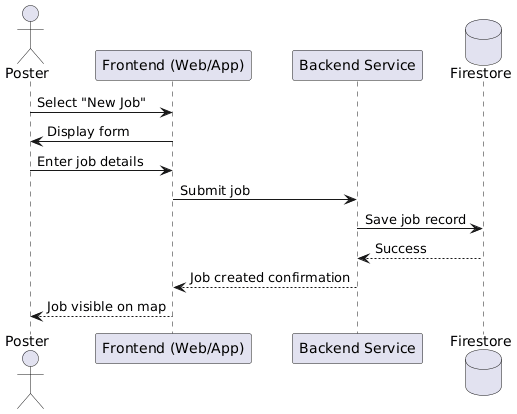
\includegraphics[width=0.9\linewidth]{UC-1.png}
  \caption{Use Case 1: Manage Jobs}
  \label{fig:uc1}
\end{figure}

\textbf{Main Flow:}
\begin{enumerate}[leftmargin=1.4em]
  \item Contractor selects ``New Job''.
  \item System prompts for title, description, category, budget type/amount, date, and location.
  \item Contractor submits; system validates and saves to database; job appears on map/list.
  \item Contractor may edit or delete until a bid is accepted.
\end{enumerate}
\textbf{Postconditions:} Job is persisted and visible to eligible bidders and \textbf{browsers}.

\subsubsection*{UC-2: Browse \& Bid (Job Bidder)}
\textbf{Actors:} Bidder \par
\textbf{Description:} Discover nearby jobs and place bids. \par
\textbf{Preconditions:} User is authenticated; KYC verified. \par

\begin{figure}[H]
  \centering
  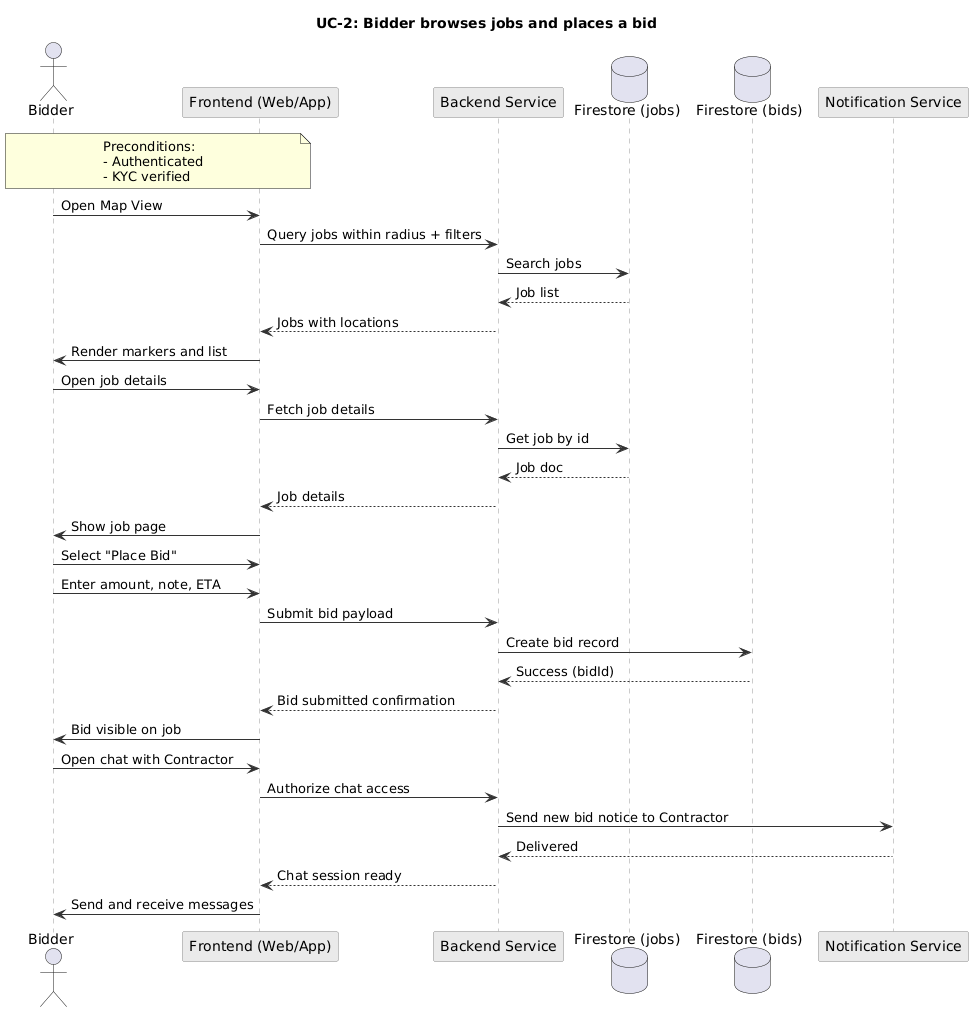
\includegraphics[width=0.9\linewidth]{UC-2.png}
  \caption{Use Case 2: Browse \& Bid}
  \label{fig:uc2}
\end{figure}

\textbf{Main Flow:}
\begin{enumerate}[leftmargin=1.4em]
  \item Bidder opens map view; system shows jobs within radius with filters.
  \item Bidder opens a job, reviews details, and selects ``Place Bid''.
  \item Bidder enters amount, note, and ETA; system validates and saves bid.
  \item Bidder can chat with the Contractor after submitting a bid.
  \item Bidder can edit/withdraw bid before award.
\end{enumerate}
\textbf{Postconditions:} Bid saved and visible to the Contractor.

\subsubsection*{UC-3: Award \& Escrow (Job Poster)}
\textbf{Actors:} Contractor \par
\textbf{Description:} Compare bids, accept a winner, and fund escrow.\par
\textbf{Preconditions:} Contractor is authenticated; job has active bids; Contractor has a payment method saved.\par

\begin{figure}[H]
  \centering
  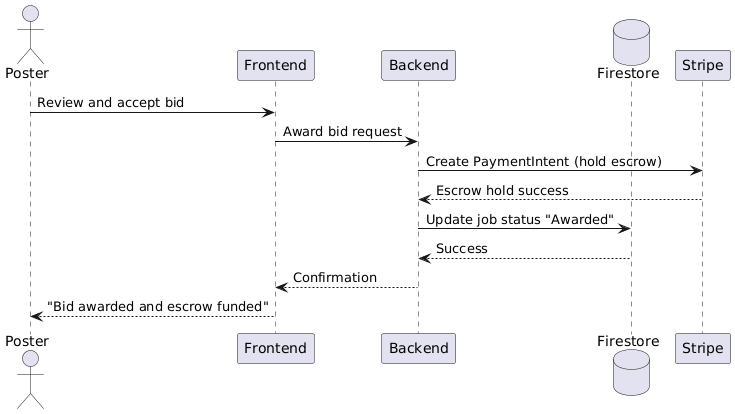
\includegraphics[width=0.9\linewidth]{UC-3.png}
  \caption{Use Case 3: Award \& Escrow}
  \label{fig:uc3}
\end{figure}

\textbf{Main Flow:}
\begin{enumerate}[leftmargin=1.4em]
  \item Contractor reviews bids (amount, ETA, ratings).
  \item Contractor accepts a bid; system creates a Stripe PaymentIntent (hold).
  \item On success, system marks job as awarded and opens thread with winner.
\end{enumerate}
\textbf{Postconditions:} Funds on hold; winner can proceed.

\subsubsection*{UC-4: Complete \& Payout}
\textbf{Actors:} Job Winner, Contractor \par
\textbf{Description:} Job Winner marks work done; Contractor confirms; funds captured and paid out.\par
\textbf{Preconditions:} Job awarded; escrow hold succeeded.\par

\begin{figure}[H]
  \centering
  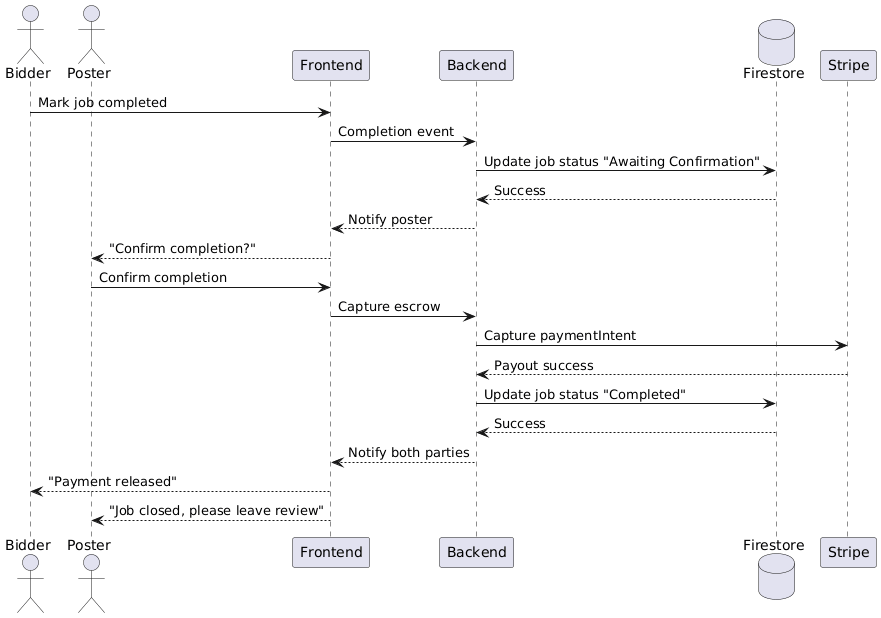
\includegraphics[width=0.9\linewidth]{UC-4.png}
  \caption{Use Case 4: Complete \& Payout}
  \label{fig:uc4}
\end{figure}

\textbf{Main Flow:}
\begin{enumerate}[leftmargin=1.4em]
  \item Job Winner marks job completed; system notifies Contractor.
  \item Contractor confirms completion (or opens dispute).
  \item On confirmation, system captures funds and pays out via Stripe Connect.
\end{enumerate}
\textbf{Postconditions:} Payment captured; both parties can review each other.


% ===================== 4. Detailed User Stories =====================
\section{Detailed User Stories}

\subsection*{Job Posters}
\paragraph{US-1: Post a New Job (High, 3 pts)}
As a \textbf{Contractor}, I want to add a job with title, description, photos, budget, date, and a map location so bidders can bid.
\begin{itemize}[leftmargin=1.4em]
  \item \textbf{Acceptance:} Required fields validated; job saved; appears on map/list; Contractor can edit/delete until award.
\end{itemize}

\paragraph{US-2: Accept a Bid \& Fund Escrow (High, 5 pts)}
As a \textbf{Contractor}, I want to accept a bid and put funds on hold so payment is guaranteed on completion.
\begin{itemize}[leftmargin=1.4em]
  \item \textbf{Acceptance:} Stripe hold succeeds; job moves to \texttt{awarded}; chat thread opens with winner.
\end{itemize}

\paragraph{US-3: Safety Score Guidance (Medium, 3 pts)}
As a \textbf{Contractor}, I want safety guidance at post-time so I can choose safer options (e.g., daylight/public meetup).
\begin{itemize}[leftmargin=1.4em]
  \item \textbf{Acceptance:} Score shown with tips; low-score flows add friction or require verification.
\end{itemize}

\paragraph{US-4: Complete KYC (High, 3 pts)}
As a \textbf{Contractor}, I want to verify my identity (document + selfie) so I can post jobs safely.
\begin{itemize}[leftmargin=1.4em]
  \item \textbf{Acceptance:} Stripe Identity flow completes; app shows verified badge; posting features unlock.
\end{itemize}

\paragraph{US-5: Duo 2FA (Medium, 2 pts)}
As a \textbf{Contractor}, I want Duo phone confirmation so my account is protected during sign-in and payouts.
\begin{itemize}[leftmargin=1.4em]
  \item \textbf{Acceptance:} 2FA challenge required; recovery path documented.
\end{itemize}

\paragraph{US-6: Job Thread Messaging (Medium, 3 pts)}
As a \textbf{Contractor}, I want a per-job chat so I can coordinate details with bidders.
\begin{itemize}[leftmargin=1.4em]
  \item \textbf{Acceptance:} Send/receive text; attachments; report/block; notifications.
\end{itemize}

\paragraph{US-7: Leave Reviews (Medium, 2 pts)}
As a \textbf{Contractor}, I want to rate and review bidders after completion so future users can trust matches.
\begin{itemize}[leftmargin=1.4em]
  \item \textbf{Acceptance:} 1–5 stars plus comment; appears on bidder profile; single review per job.
\end{itemize}

\subsection*{Job Bidders}
\paragraph{US-8: Browse Nearby Jobs (High, 3 pts)}
As a \textbf{bidder}, I want to see jobs near me with filters so I can quickly find relevant work.
\begin{itemize}[leftmargin=1.4em]
  \item \textbf{Acceptance:} Map/list render; radius/category/budget/date filters; open job details view.
\end{itemize}

\paragraph{US-9: Place a Bid (High, 5 pts)}
As a \textbf{bidder}, I want to place a bid with amount, note, and ETA so the Contractor can evaluate me.
\begin{itemize}[leftmargin=1.4em]
  \item \textbf{Acceptance:} Bid saved; Contractor notified; bidder can edit/withdraw prior to award.
\end{itemize}

\paragraph{US-10: Complete KYC (High, 3 pts)}
As a \textbf{bidder}, I want to verify my identity (document + selfie) so I can bid on jobs safely.
\begin{itemize}[leftmargin=1.4em]
  \item \textbf{Acceptance:} Stripe Identity flow completes; app shows verified badge; bidding features unlock.
\end{itemize}

\paragraph{US-11: Duo 2FA (Medium, 2 pts)}
As a \textbf{bidder}, I want Duo phone confirmation so my account is protected during sign-in and payouts.
\begin{itemize}[leftmargin=1.4em]
  \item \textbf{Acceptance:} 2FA challenge required; recovery path documented.
\end{itemize}

\paragraph{US-12: Job Thread Messaging (Medium, 3 pts)}
As a \textbf{bidder}, I want a per-job chat so I can coordinate details with Contractor.
\begin{itemize}[leftmargin=1.4em]
  \item \textbf{Acceptance:} Send/receive text; attachments; report/block; notifications.
\end{itemize}

\paragraph{US-13: Leave Reviews (Medium, 2 pts)}
As a \textbf{bidder}, I want to rate and review Contractor after completion so future users can trust matches.
\begin{itemize}[leftmargin=1.4em]
  \item \textbf{Acceptance:} 1–5 stars plus comment; appears on Contractor profile; single review per job.
\end{itemize}

\subsection*{Job Browsers (Not KYC-Verified Users)}
\paragraph{US-14: Browse Jobs Read-Only (Medium, 2 pts)}
As a \textbf{browser}, I want to explore posted jobs on a map in read-only mode, so I can understand the platform's services before committing.
\begin{itemize}[leftmargin=1.4em]
  \item \textbf{Acceptance:} Map/list view available; limited job details visible; registration prompt when trying to post/bid.
\end{itemize}

\paragraph{US-15: View Limited Job Details (Medium, 1 pt)}
As a \textbf{browser}, I want to view limited job details (e.g., title, category, approximate location, budget range) without registering, so I see the platform's value.
\begin{itemize}[leftmargin=1.4em]
  \item \textbf{Acceptance:} Basic job info visible; contact details and full descriptions hidden; registration required for full access.
\end{itemize}

\paragraph{US-16: Registration Prompt (Medium, 1 pt)}
As a \textbf{browser}, I want to be prompted to create an account if I try to post a job or place a bid, so I know registration is required.
\begin{itemize}[leftmargin=1.4em]
  \item \textbf{Acceptance:} Clear registration modal appears; KYC/2FA requirements explained; seamless signup flow.
\end{itemize}

\paragraph{US-17: KYC/2FA Instructions (Medium, 1 pt)}
As a \textbf{newly registered user}, I want clear instructions that I must complete KYC verification and enable Duo 2FA before being allowed to post jobs or bid, so I understand the trust policy.
\begin{itemize}[leftmargin=1.4em]
  \item \textbf{Acceptance:} Step-by-step guidance; progress indicators; help resources available.
\end{itemize}

\paragraph{US-18: Access Support Resources (Low, 1 pt)}
As a \textbf{browser}, I want access to support or FAQ pages, so I can ask questions or learn more before verifying my account.
\begin{itemize}[leftmargin=1.4em]
  \item \textbf{Acceptance:} Support contact form; FAQ section; help documentation accessible without full registration.
\end{itemize}

\subsection*{Admin}
\paragraph{US-19: Review Reports (High, 3 pts)}
As an \textbf{admin}, I want to review user reports and disputes so I can maintain platform safety and integrity.
\begin{itemize}[leftmargin=1.4em]
  \item \textbf{Acceptance:} Report dashboard; case management tools; resolution tracking.
\end{itemize}

\paragraph{US-20: Manage Categories (Medium, 2 pts)}
As an \textbf{admin}, I want to manage job categories so the platform stays organized and relevant.
\begin{itemize}[leftmargin=1.4em]
  \item \textbf{Acceptance:} Category CRUD operations; validation; audit logging.
\end{itemize}

\paragraph{US-21: Handle Disputes (High, 4 pts)}
As an \textbf{admin}, I want to handle payment and job disputes so conflicts are resolved fairly.
\begin{itemize}[leftmargin=1.4em]
  \item \textbf{Acceptance:} Dispute intake; evidence review; resolution workflow; communication tools.
\end{itemize}

\paragraph{US-22: System Monitoring (Medium, 2 pts)}
As an \textbf{admin}, I want to monitor system health and performance so I can ensure platform reliability.
\begin{itemize}[leftmargin=1.4em]
  \item \textbf{Acceptance:} Dashboard with metrics; alert system; performance monitoring.
\end{itemize}

% ===================== 5. Documentation Updates =====================
\section{Documentation Updates}

\subsection{System Architecture (Prototype)}
\textbf{Frontend:} React + SCSS (Firebase Hosting)\\
\textbf{Backend:} Node.js + Express (Firebase Functions or Cloud Run)\\
\textbf{Database:} Firebase Firestore (NoSQL, real-time)\\
\textbf{Storage:} Firebase Cloud Storage\\
\textbf{Auth:} Firebase Auth (OAuth, email+password) + Duo 2FA; KYC via Stripe Identity\\
\textbf{Payments:} Stripe Connect (escrow)\\
\textbf{Maps:} Google Maps JS, Places, Geocoding, Distance Matrix

\subsection{Planning Document and Log}
\begin{itemize}[leftmargin=1.4em]
  \item \textbf{Changes from Iteration~1.1:} Committed to Firebase stack; clarified escrow flow; added explicit safety score gating.
  \item \textbf{Plan Delta:} Pulled reviews into Iteration 2 tail; background checks remain later.
\end{itemize}

% ===================== 6. Iteration Plan and Backlog =====================
\section{Iteration Plan and Backlog}

\subsection{Iteration Plan (Weeks 6--10)}
\textbf{Full iteration plan can be found in documentation/1.1 Project Proposal/main.pdf in the project repo.}
\begin{itemize}[leftmargin=1.4em]
  \item \textbf{Weeks 6-7:} Finalize functional requirements; implement US-1 (post job) and US-8 (browse jobs); Firestore rules draft.
  \item \textbf{Weeks 8-9:} Implement US-9 (place bid) and US-2 (accept bid \& escrow stub); basic messaging skeleton.
  \item \textbf{Week 10:} Review feedback; refine UX; stabilize prototype; add US-6/US-12 (chat MVP) and US-7/US-13 (reviews, stub).
\end{itemize}

\subsection{Updated Backlog (Top)}
\begin{longtable}{@{}p{0.16\linewidth} p{0.52\linewidth} p{0.12\linewidth} p{0.12\linewidth}@{}}
\toprule
\textbf{ID} & \textbf{Story} & \textbf{Priority} & \textbf{Pts} \\
\midrule
US-1 & Post a new job & High & 3 \\
US-2 & Accept bid \& fund escrow & High & 5 \\
US-8 & Browse nearby jobs & High & 3 \\
US-9 & Place a bid & High & 5 \\
US-4 & Complete KYC (Contractor) & High & 3 \\
US-10 & Complete KYC (Bidder) & High & 3 \\
US-5 & Duo 2FA (Contractor) & Medium & 2 \\
US-11 & Duo 2FA (Bidder) & Medium & 2 \\
US-3 & Safety score guidance & Medium & 3 \\
US-6 & Job thread messaging (Contractor) & Medium & 3 \\
US-12 & Job thread messaging (Bidder) & Medium & 3 \\
US-7 & Leave reviews (Contractor) & Medium & 2 \\
US-13 & Leave reviews (Bidder) & Medium & 2 \\
US-14 & Browse jobs read-only (Browser) & Medium & 2 \\
US-15 & View limited job details (Browser) & Medium & 1 \\
US-16 & Registration prompt (Browser) & Medium & 1 \\
US-17 & KYC/2FA instructions (Browser) & Medium & 1 \\
US-18 & Access support resources (Browser) & Low & 1 \\
US-19 & Review reports (Admin) & High & 3 \\
US-20 & Manage categories (Admin) & Medium & 2 \\
US-21 & Handle disputes (Admin) & High & 4 \\
US-22 & System monitoring (Admin) & Medium & 2 \\
\bottomrule
\end{longtable}

% ===================== 7. Submission Guidelines =====================
\section{Submission Guidelines}
\begin{itemize}[leftmargin=1.4em]
  \item \textbf{GitHub Repository:} Push prototype code and documentation; tag release as \texttt{ITR1.2}.
  \item \textbf{eClass Submission:} Submit one PDF containing: Requirements; Use Case Diagram \& Descriptions; Detailed User Stories; Initial Prototype Overview; Updated Plan and Backlog.
\end{itemize}

% ===================== Appendix A: API Inventory =====================
\section*{Appendix A: API Inventory (Condensed)}
\begin{longtable}{@{}p{0.32\linewidth} p{0.64\linewidth}@{}}
\toprule
\textbf{Area} & \textbf{APIs / Notes} \\
\midrule
Auth/Identity & Firebase Auth (OAuth, email+password); Duo 2FA; Stripe Identity (KYC) \\
Payments & Stripe Connect (escrow), Webhooks, Radar \\
Maps/Geo & Google Maps JS; Places Autocomplete/Details; Geocoding; Distance Matrix \\
Notifications & Firebase Cloud Messaging; Twilio SMS + Proxy \\
Storage & Firebase Cloud Storage \\
Analytics/Ops & PostHog; Sentry; OpenTelemetry \\
\bottomrule
\end{longtable}

% ===================== Appendix B: Firestore Schema =====================
\section*{Appendix B: Firestore Schema (Indicative)}
\begin{lstlisting}[language=json,caption={Firestore Collections \& Example Documents}]
/users/{userId}
{
  "name": "string",
  "email": "string",
  "phone": "string",
  "avatarUrl": "string",
  "isBidder": true,
  "kycStatus": "pending" | "verified" | "failed",
  "duoEnabled": true,
  "createdAt": "timestamp",
  "updatedAt": "timestamp"
}

/jobs/{jobId}
{
  "contractorID": "users/{userId}",
  "title": "string",
  "description": "string",
  "category": "string",
  "budgetType": "fixed" | "open",
  "budgetAmount": 120.50,
  "location": { "lat": 43.6426, "lng": -79.3871, "address": "string" },
  "desiredDate": "timestamp",
  "status": "open" | "awarded" | "in_progress" | "completed" | "cancelled",
  "createdAt": "timestamp",
  "updatedAt": "timestamp"
}

/bids/{bidId}
{
  "jobId": "jobs/{jobId}",
  "bidderId": "users/{userId}",
  "amount": 95.00,
  "note": "string",
  "etaHours": 6,
  "status": "active" | "declined" | "accepted" | "cancelled",
  "createdAt": "timestamp"
}

/messages/{messageId}
{
  "jobId": "jobs/{jobId}",
  "senderId": "users/{userId}",
  "body": "string",
  "attachmentUrl": "string",
  "createdAt": "timestamp"
}

/reviews/{reviewId}
{
  "jobId": "jobs/{jobId}",
  "raterId": "users/{userId}",
  "rateeId": "users/{userId}",
  "rating": 5,
  "comment": "string",
  "createdAt": "timestamp"
}
\end{lstlisting}

\end{document}
